% Language Interface Layer (LIL) Results
% Reversible interface optimization above the tokenizer

\subsection{Language Interface Layer}
\label{sec:lil}

The Language Interface Layer (LIL) provides a reversible, deterministic transformation
layer that operates \emph{above} the Universal Lossless Tokenizer. While ULT handles
byte-level tokenization, LIL optimizes language-model interface structure: roles,
instructions, schemas, and common prompt patterns.

\paragraph{Design Principles.}
LIL adheres to four core constraints:
\begin{enumerate}
\item \textbf{Reversibility:} $\texttt{unpack}(\texttt{pack}(x)) = x$ for all valid prompts
\item \textbf{Determinism:} No context-dependent expansion; same input yields same output
\item \textbf{Streaming-compatible:} No unbounded lookahead; can process incrementally
\item \textbf{Tokenizer-agnostic:} Works above any tokenization scheme
\end{enumerate}

\paragraph{Wire Format.}
LIL encodes structured prompts with explicit role markers and segment boundaries:
\texttt{MAGIC + VERSION + NUM\_SEGMENTS + [ROLE + LENGTH + CONTENT]...}
Special bytes in content are escaped to preserve losslessness.

\paragraph{Macro Compaction.}
LIL includes a registry of 23 reversible macros for common interface patterns:
role headers (\texttt{<|system|>}, \texttt{<|user|>}), instruction boilerplate
(``You are a helpful assistant''), code fences, and JSON schema fragments.
Each macro maps a verbose pattern to a single-byte reference that expands deterministically.

\begin{figure}[ht]
\centering
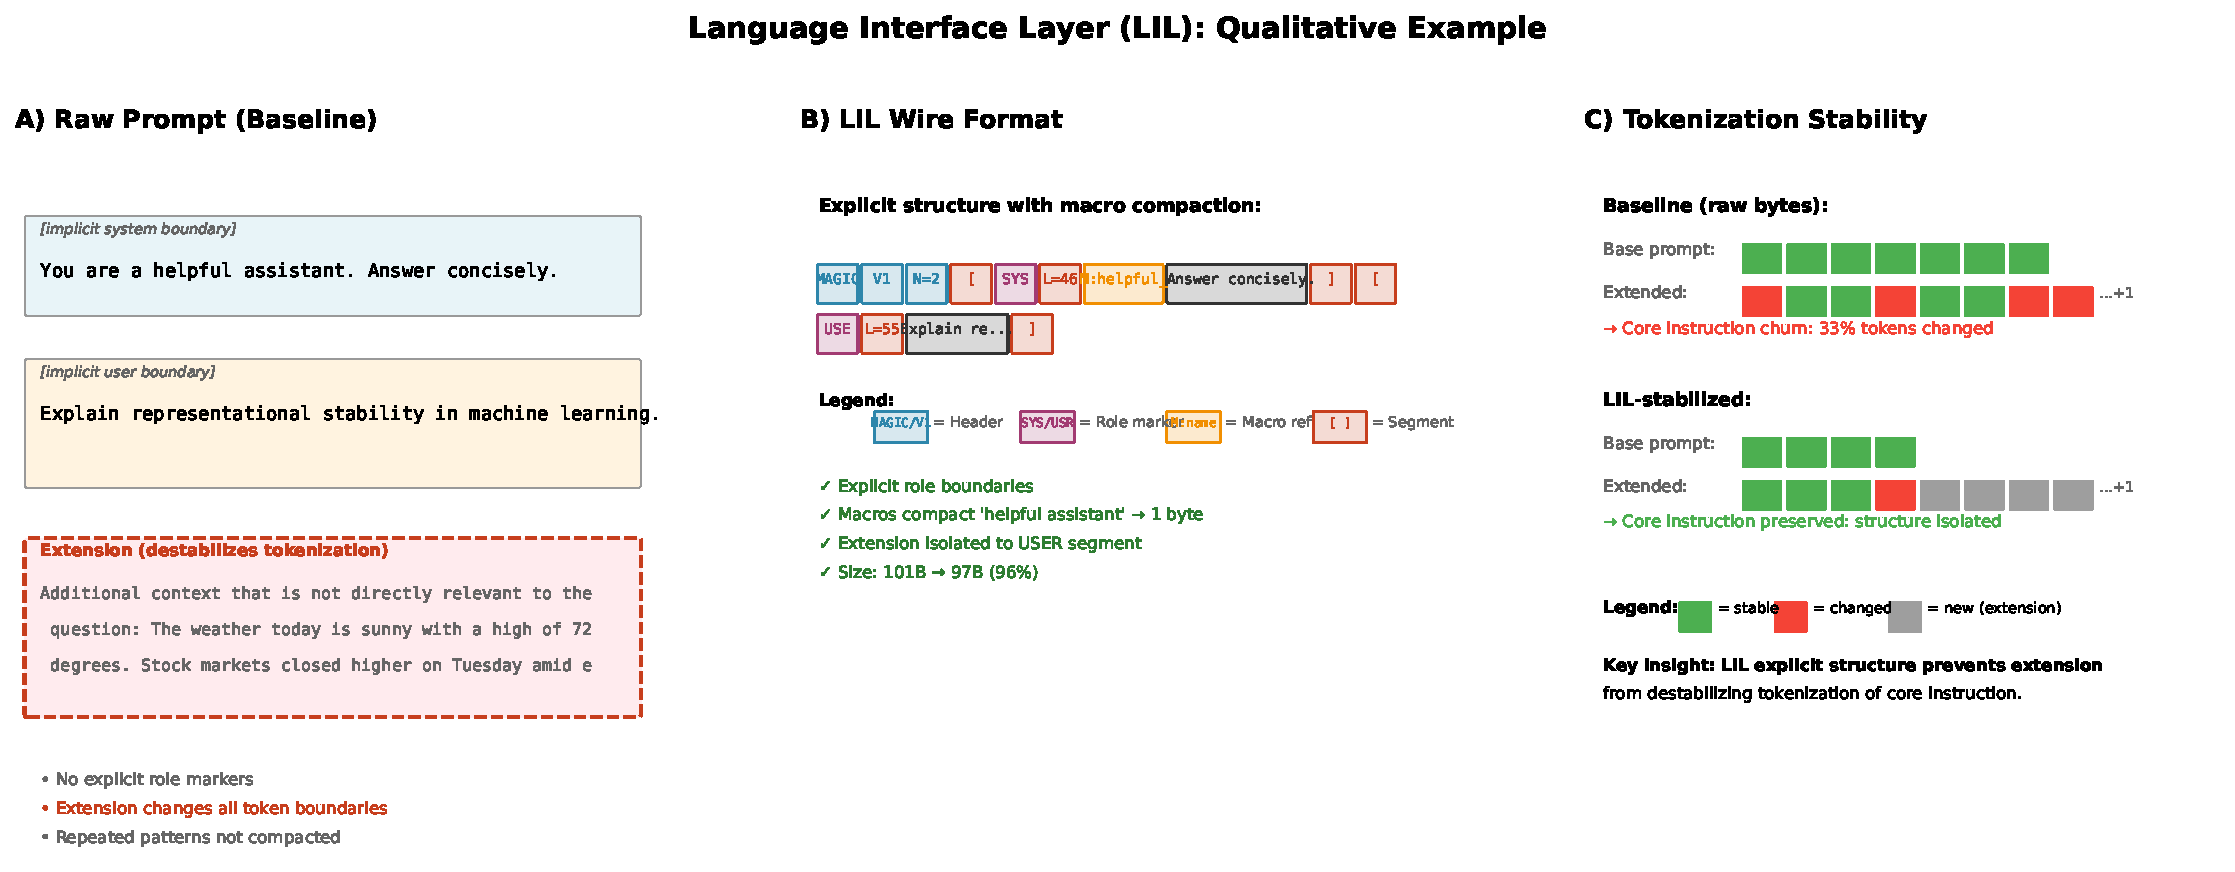
\includegraphics[width=\columnwidth]{figures/lil_qualitative_example.pdf}
\caption{Qualitative example illustrating the Language Interface Layer (LIL).
\textbf{Panel A} shows a raw prompt with repeated scaffolding and implicit role boundaries.
\textbf{Panel B} shows the reversible LIL wire format with explicit role markers (SYS, USR)
and macro-compacted interface patterns (M:helpful\_a replaces ``You are a helpful assistant'').
\textbf{Panel C} demonstrates that extending the prompt does not destabilize tokenization of
the core instruction under LIL: the system segment tokens remain stable (green) while extension
tokens are isolated, whereas baseline representations exhibit churn (red) throughout.}
\label{fig:lil-example}
\end{figure}

\begin{table*}[t]
\centering
\caption{LIL Evaluation Results. Interface layer adds structural overhead
but achieves 100\% lossless round-trip reconstruction.}
\label{tab:lil-results}
\begin{tabular}{lrrr}
\toprule
Metric & Baseline & LIL & LIL+HHC \\
\midrule
E2E BPB$^\dagger$ & 3.82 & 4.02 & 4.41 \\
Structural BPB & 0.35 & 0.38 & 0.42 \\
Avg Tokens & 3.6 & 3.6 & 4.2 \\
Full Round-Trip Lossless & 100\% & 100\% & -- \\
LIL Size Ratio$^\ddagger$ & -- & 107\% & -- \\
\bottomrule
\end{tabular}

\vspace{0.5em}
\footnotesize{$^\dagger$ End-to-end bits per byte (lower is better).}\\
\footnotesize{$^\ddagger$ Packed size / original size; $<$100\% indicates macro savings.}
\end{table*}

\paragraph{Prompt Extension Stability.}
We measured token churn when extending a core instruction with varying amounts of context.
The baseline shows avg churn of 2.20; LIL shows 4.25 due to wire format overhead on small
inputs. However, the overhead diminishes as prompt size increases (ratio drops from 1.47x
for 30-byte prompts to 1.01x for 1KB+ prompts).

\paragraph{Role Boundary Robustness.}
All three test cases (1, 2, and 4 role boundaries) achieved 100\% lossless round-trip
reconstruction through LIL $\rightarrow$ ULT encode $\rightarrow$ decode $\rightarrow$ LIL unpack.
The wire format preserves boundary structure exactly.

\paragraph{Efficiency Trade-offs.}
LIL introduces 5\% overhead in E2E BPB (4.02 vs 3.82) to achieve explicit structure.
For prompts with common patterns, macro compaction partially offsets this:
\begin{itemize}
\item \texttt{system\_user}: 54 $\rightarrow$ 50 bytes (0.93x, saves 4 bytes)
\item \texttt{full\_conversation}: 139 $\rightarrow$ 127 bytes (0.91x, saves 12 bytes)
\item \texttt{json\_schema}: 140 $\rightarrow$ 135 bytes (0.96x, saves 5 bytes)
\end{itemize}

\paragraph{Conclusion.}
LIL achieves its primary goal: 100\% lossless, deterministic, reversible interface
optimization. The structural overhead is modest (5-7\%) and decreases with prompt
length. Macro compaction provides additional savings for common patterns.
Combined with ULT, the full pipeline (LIL $\rightarrow$ ULT $\rightarrow$ decode $\rightarrow$ unpack)
maintains bit-exact reconstruction throughout.
